\documentclass[UTF8]{ctexart}
\usepackage{lmodern}
\usepackage{amsmath}
\usepackage{graphicx}
\usepackage{float}%提供float浮动环境
\usepackage{booktabs}%提供命令\toprule、\midrule、\bottomrule
\usepackage{geometry}

% \begin{figure}[htbp]
%     \centering
%     \includegraphics[width=0.60\textwidth]{}
% \end{figure}

% \begin{table}[H]
%     \centering
%     \caption{\label{表}\textbf{}}
%     \begin{tabular}{ccc}
%     \toprule

%     \midrule
          
%     \bottomrule
%     \end{tabular}
% \end{table}

\geometry{a4paper,left=2cm,right=2cm,top=2cm,bottom=2cm}

\title{{电子技术基础实验} \\ \textbf{实验三\ 三极管放大电路2}}
\author{\\\textbf{祝尔乐}
        \\\textbf{未央-电01}
        }
\date{\textbf{\today}}

\begin{document}
\maketitle

\section*{一.实验目的}
\subsubsection*{1、了解差分放大电路的特性和工作原理。}

\subsubsection*{2、熟悉差分放大电路的设计和调试方法。}

\subsubsection*{3、熟悉用 LTspice 仿真电路。}


\section*{二.实验内容}

\subsection*{1.测量差分放大电路的参数}
\begin{figure}[htbp]
    \centering
    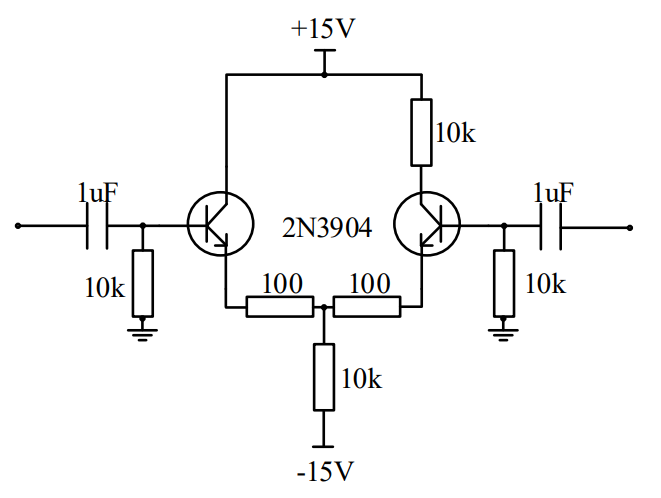
\includegraphics[width=0.60\textwidth]{电路图1.png}
    \caption{电路图1}
\end{figure}

按照电路图1所示电路连接电路。

\subsubsection*{(1)测量放大电路中三极管的静态集电极电流及电压,并与理论及仿真结
果比较}
记左右两端的三极管分别为$T1$,$T2$。
先求解理论值。由三极管特性,$\beta$取200,有

\begin{align}
    \nonumber
    U_{B1} &= - I_{B1} \cdot 10k \\
    \nonumber
    U_{B2} &= - I_{B2} \cdot 10k \\
    \nonumber
    U_{E1} &= I_{E1} \cdot 100 + (I_{E1} + I_{E2}) \cdot 10k - 15\\
    \nonumber
    U_{E2} &= I_{E2} \cdot 100 + (I_{E1} + I_{E2}) \cdot 10k - 15\\
    \nonumber
    I_{E1} &= (\beta + 1) I_{B1} \approx \beta I_{B1}\\
    \nonumber
    I_{E2} &= (\beta + 1) I_{B2} \approx \beta I_{B2}\\
    \nonumber
    U_{B1} &\approx U_{E1} + 0.7\\
    \nonumber
    U_{B2} &\approx U_{E2} + 0.7
\end{align}

解得
\begin{align}
    \nonumber
    I_{B1} &= I_{B2} \approx 3.57 \mu A \\
    \nonumber
    I_{C1} &= I_{C2} \approx I_{E1} = I_{E2} \approx 0.71 mA\\
    \nonumber
    U_{C1} &= 15V\\
    \nonumber
    U_{C2} &= 15 - I_{C1}\cdot 10k \approx 7.9V
\end{align}

仿真结果如下:

\begin{figure}[htbp]
    \centering
    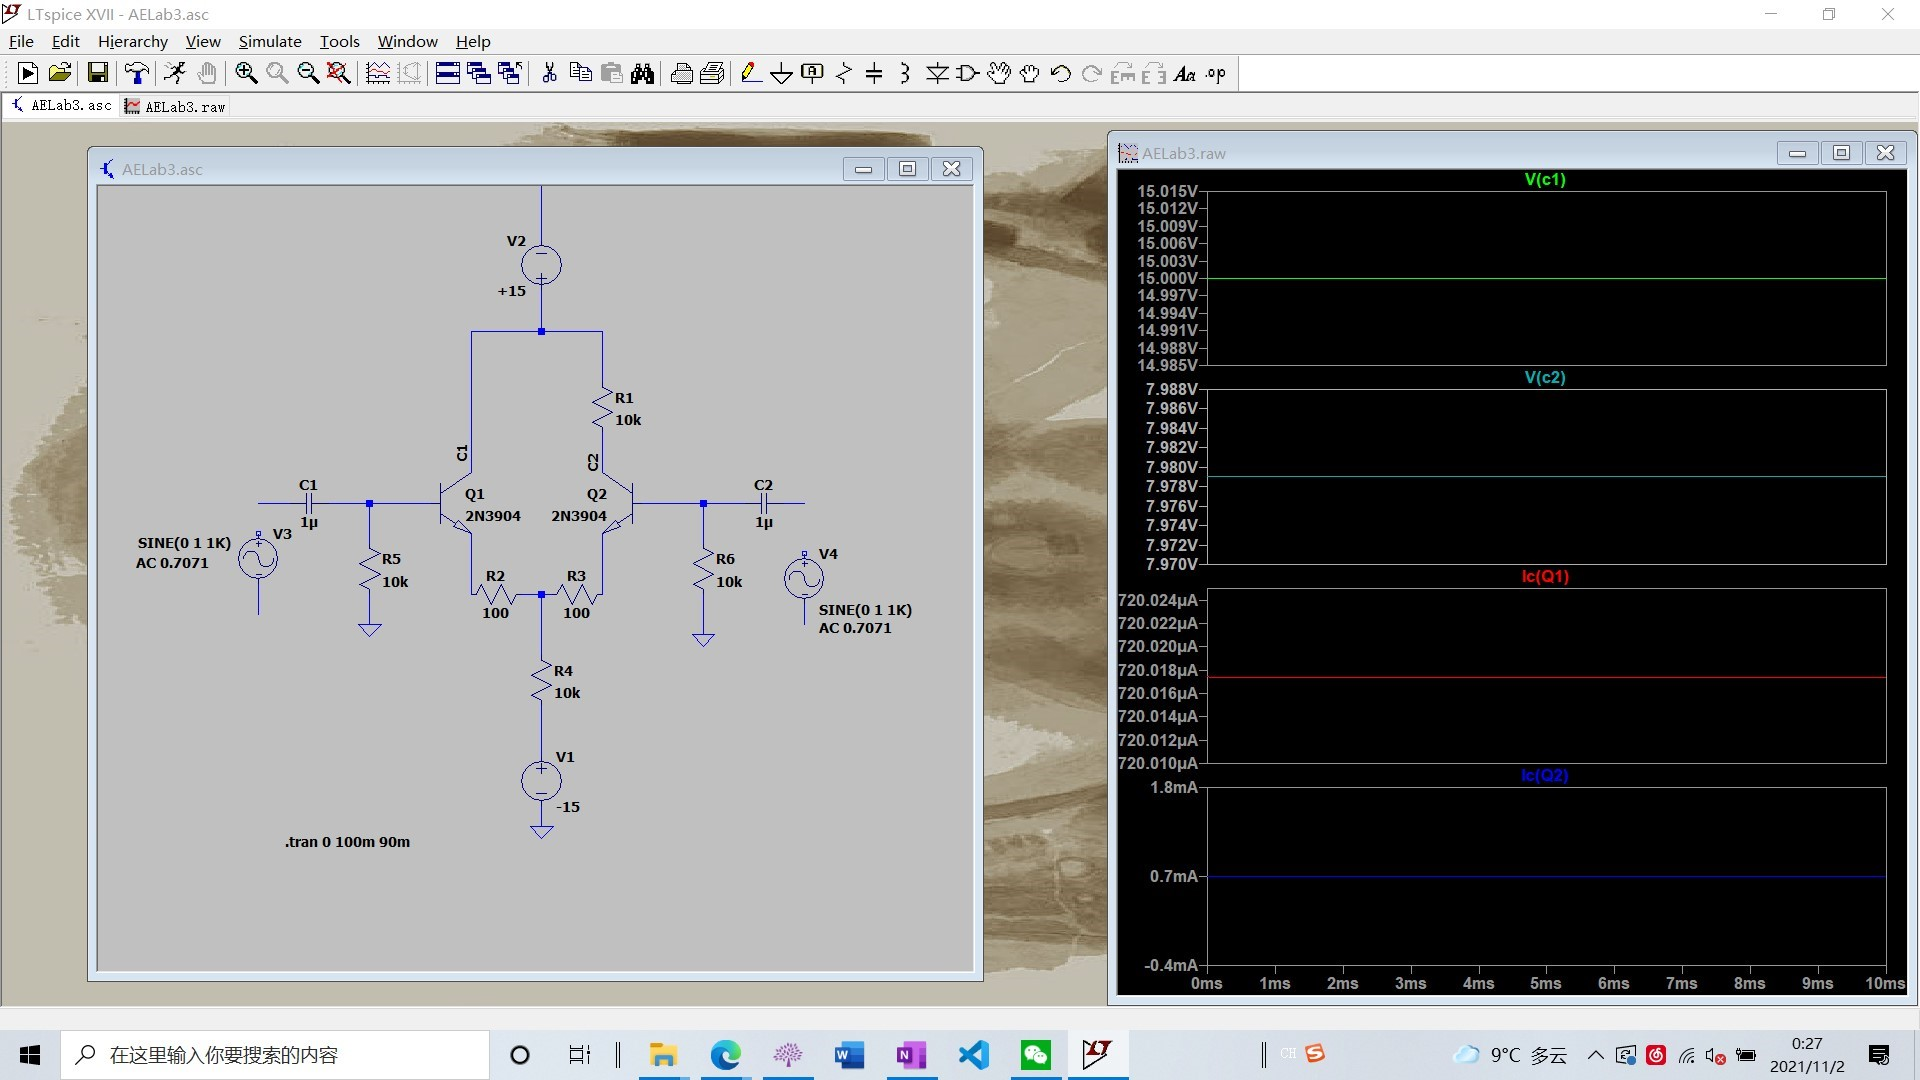
\includegraphics[width=0.60\textwidth]{1-1-静态.jpg}
\end{figure}

可见,与理论估算结果相近。

连接电路后进行测量,实际测量结果为:

\begin{table}[H]
    \centering
    \caption{\label{表1}\textbf{集电极电流与电压}}
    \begin{tabular}{cccc}
    \toprule
        $U_{C1}/V$ & $I_{C1}/mA$ & $U_{C2}/V$ & $I_{C2}/mA$ \\
    \midrule
        15.21 & 0.73 & 8.26 & 0.68 \\
    \bottomrule
    \end{tabular}
\end{table}

实际测量结果中,由于输出电压比设定电压偏大,所以电压测量值偏大。总体而言,
测量值与理论值和仿真值相近。

\subsubsection*{(2)测量放大电路的差模和共模增益,并与仿真结果比较}

设定信号频率为$100Hz$,输入信号为两个大小为$5mVrms$的正弦波,相位差分别设为
$0^o$(共模)和$180^o$(差模)。
仿真结果如下:
\begin{figure}[htbp]
    \centering
    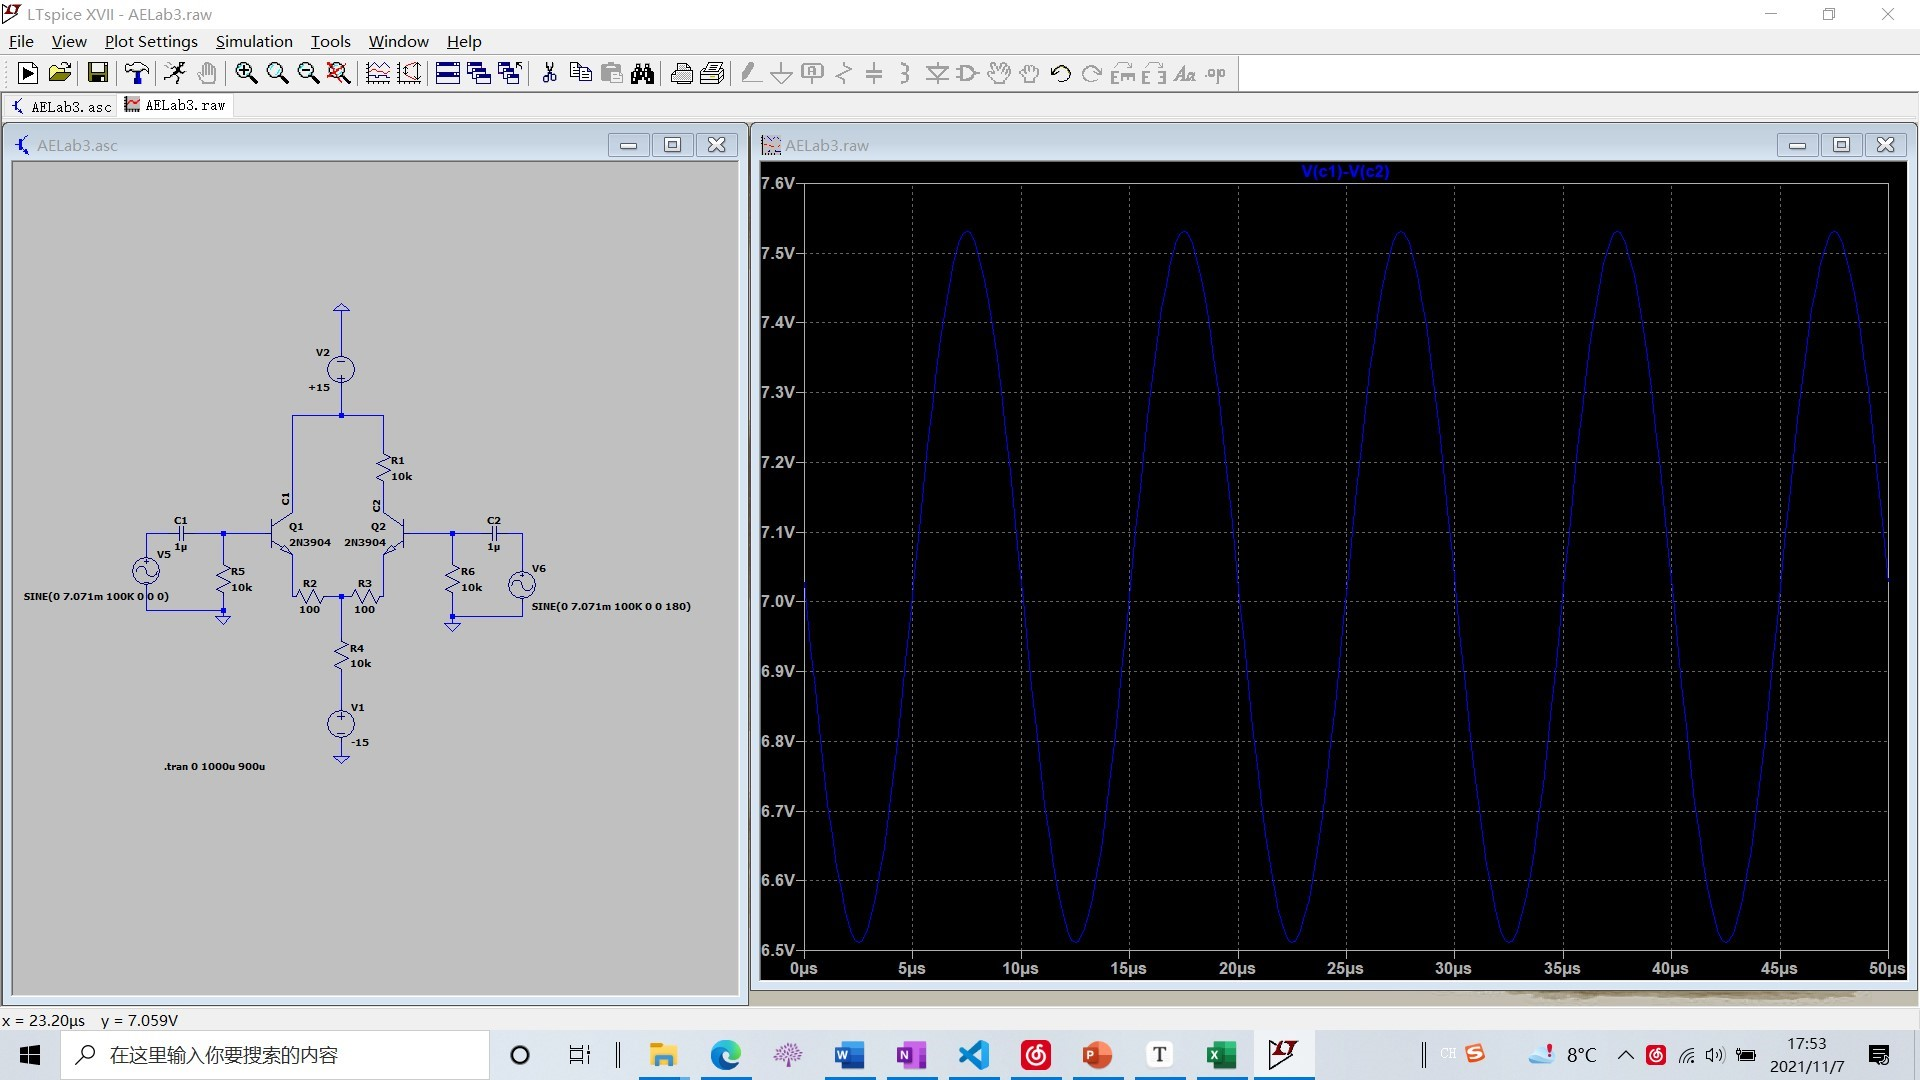
\includegraphics[width=0.60\textwidth]{1-2-差模.jpg}
\end{figure}

\begin{figure}[htbp]
    \centering
    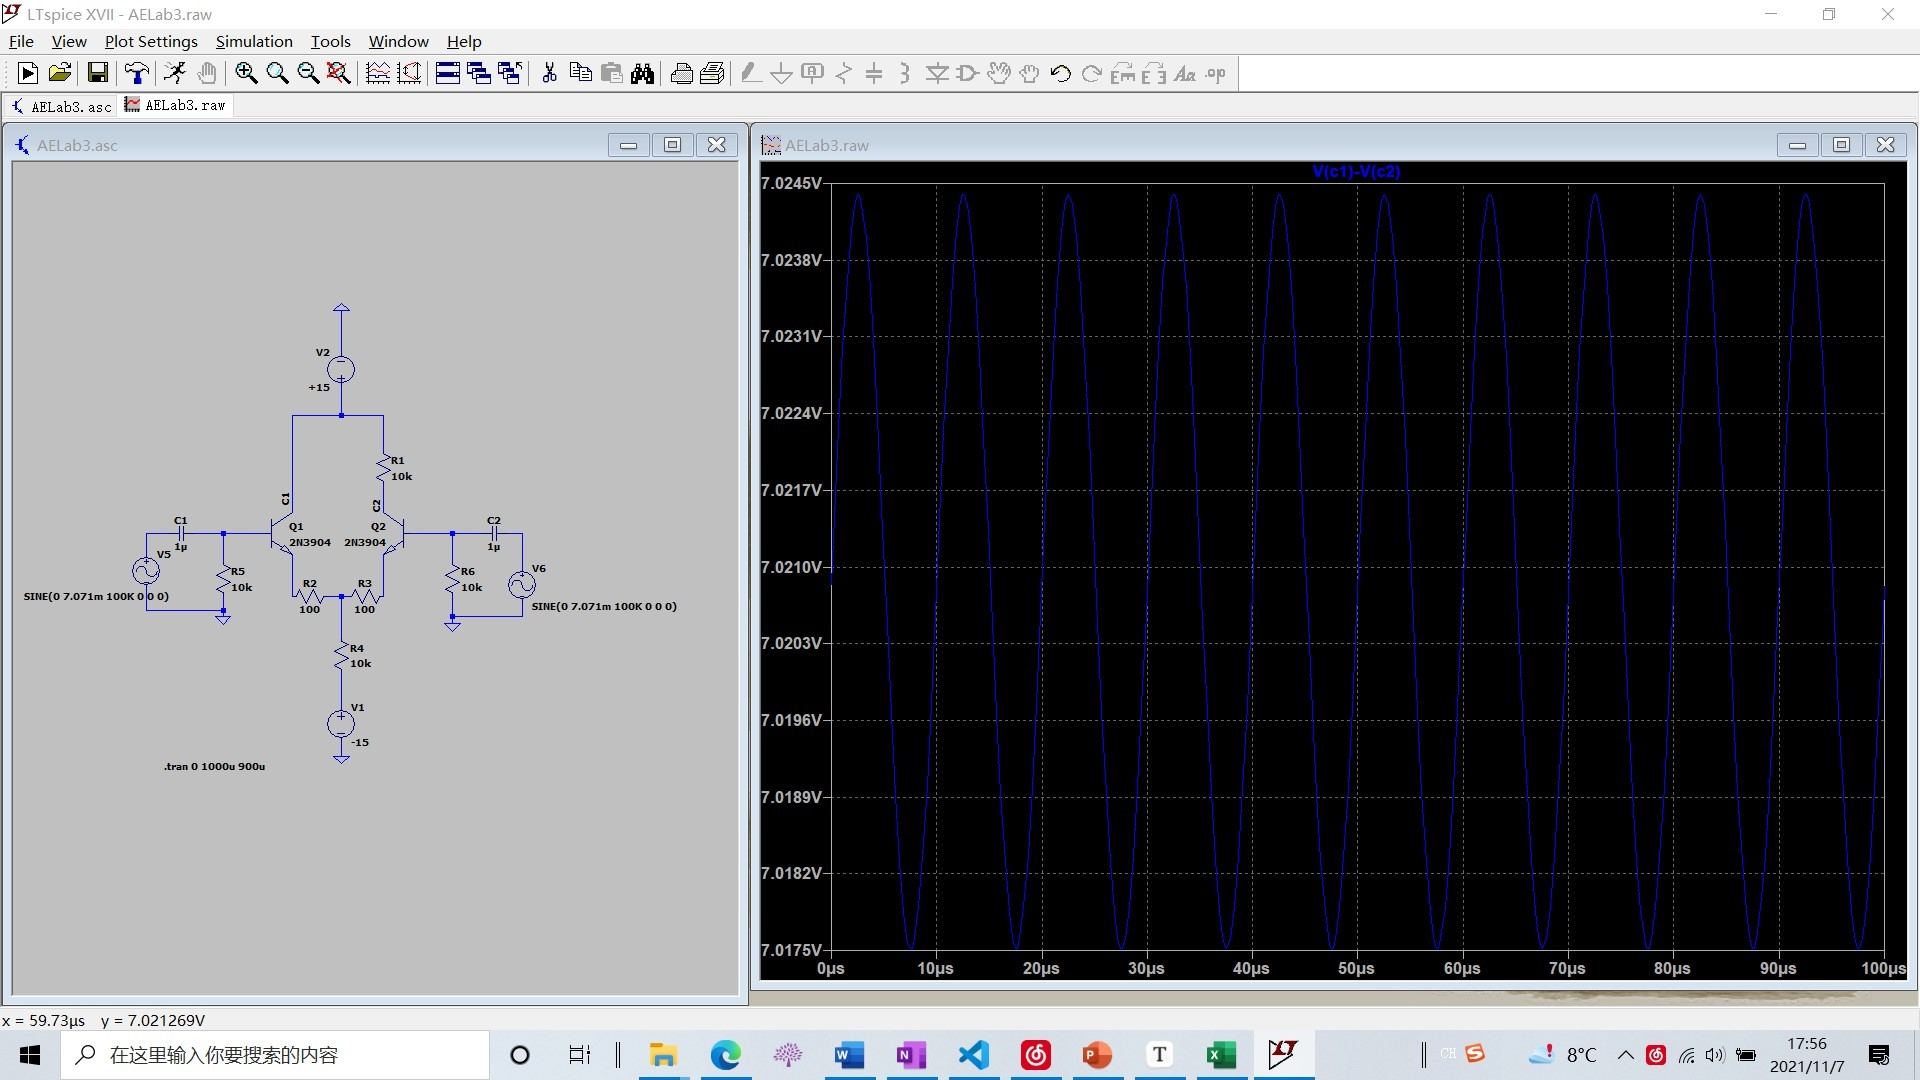
\includegraphics[width=0.60\textwidth]{1-3-共模.jpg}
\end{figure}

仿真得到的差模输出信号为$1022mV$,共模输出信号约为$6.9mV$。

测量输出电压的峰峰值$U_{Od,pp},U_{Oc,pp}$,使用$A = \frac{U_{O,pp}}{2\sqrt{2} \cdot 5m}$
计算出放大倍数$A_d, A_c$。

测量结果和计算结果如下表:

\begin{table}[H]
    \centering
    \caption{\label{表2}\textbf{共模和差模放大倍数}}
    \begin{tabular}{cccc}
    \toprule
        $U_{Od}/mVPP$ & $A_d$ & $U_{Oc}/mVPP$ & $A_c$\\
    \midrule
        976 & 69.0 & 59.2 & 4.2 \\
    \bottomrule
    \end{tabular}
\end{table}

测量结果中共模信号放大倍数与仿真结果相差较大,可能是电路的实际特性
与仿真参数的差异引起的。

\subsubsection*{(3)测量放大电路增益的幅频特性,并与仿真结果比较}

输入电压依旧采用两个$5mVrms$,相角差为$180^o$的正弦交流电源。频率从10Hz变化到100kHz。

对幅频特性进行仿真:

\begin{figure}[htbp]
    \centering
    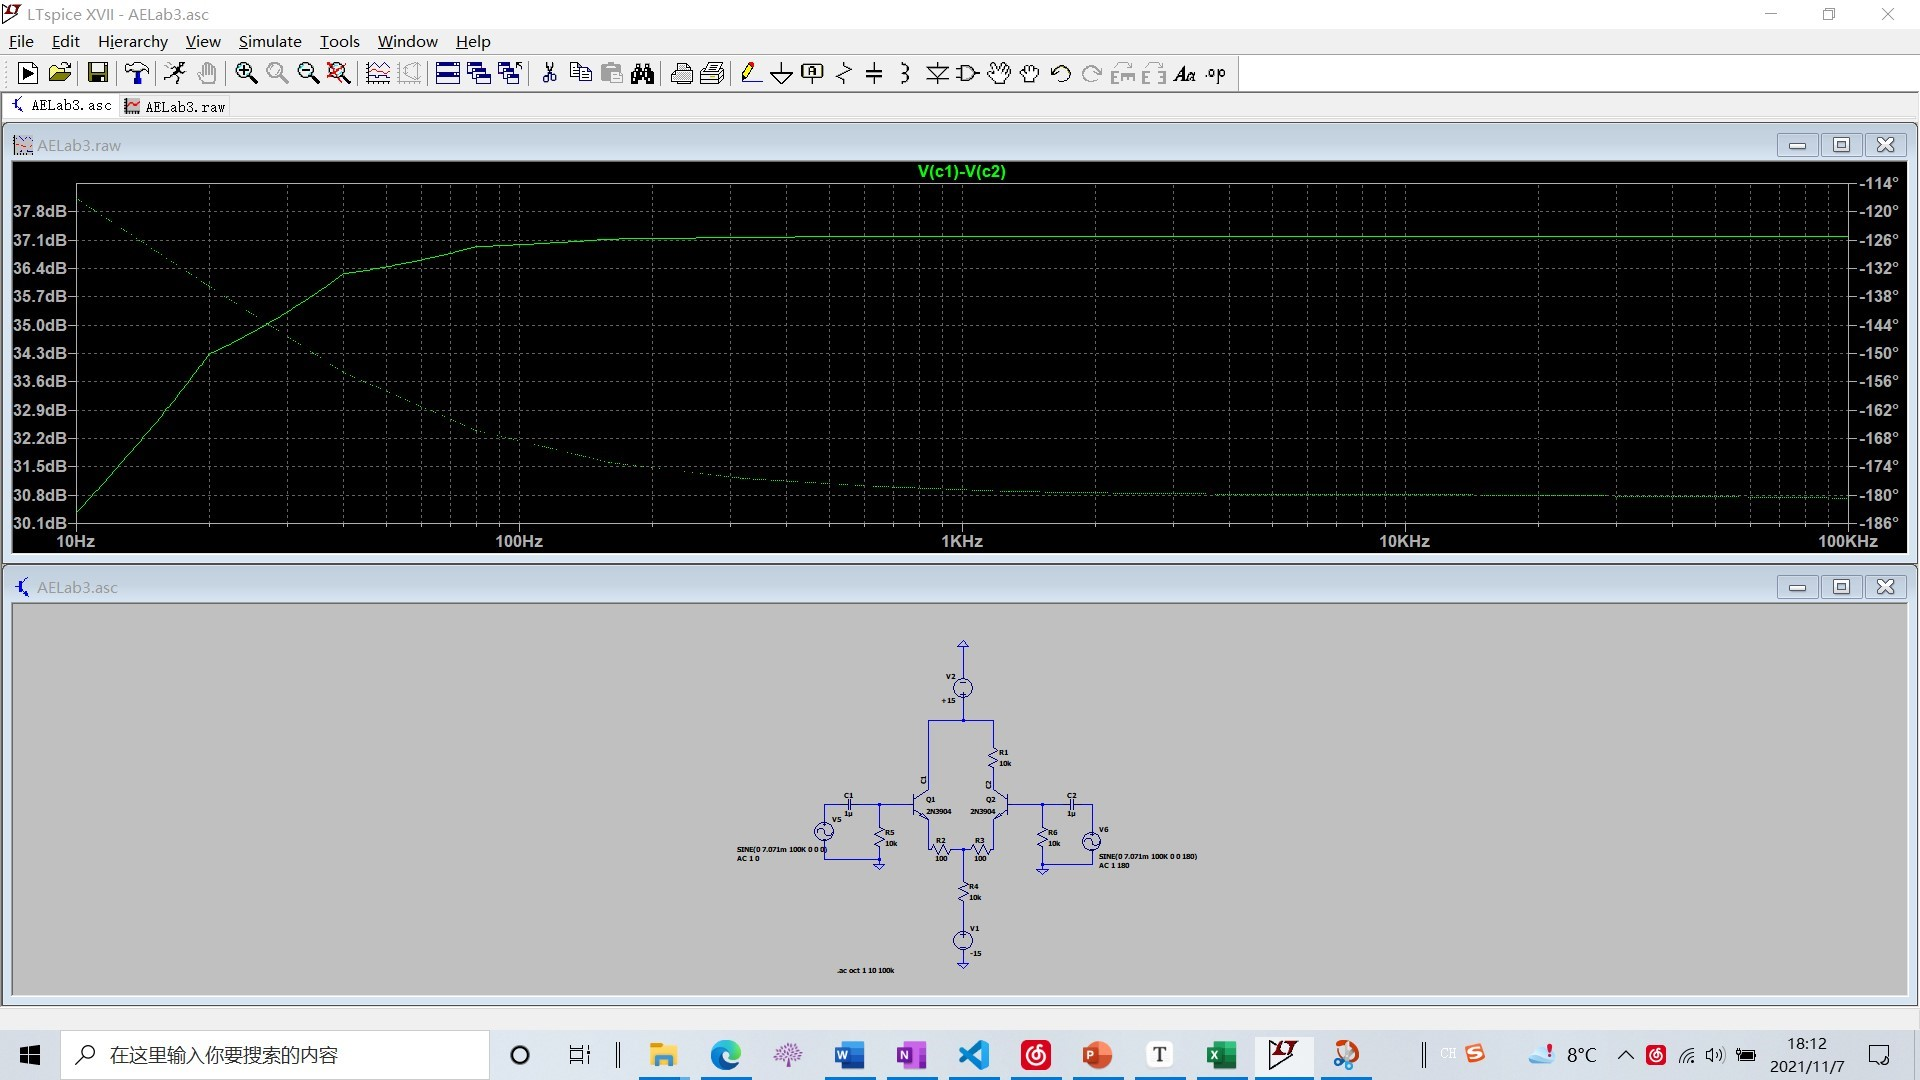
\includegraphics[width=0.60\textwidth]{1-3-幅频特性.jpg}
\end{figure}

\newpage
实验中的测量结果如下表:

\begin{table}[H]
    \centering
    \caption{\label{表3}\textbf{幅频特性}}
    \begin{tabular}{ccccccccc}
    \toprule
        $f/Hz$ & 10 & 20 & 40 & 70 & 100 & 1k & 10k & 100k\\
    \midrule
         $U_{o}/VPP$ & 0.175 & 0.342 & 0.564 & 0.684 & 0.805 & 1.02 & 1.14 & 1.06\\ 
    \bottomrule
    \end{tabular}
\end{table}

画出幅频特性:
\begin{figure}[htbp]
    \centering
    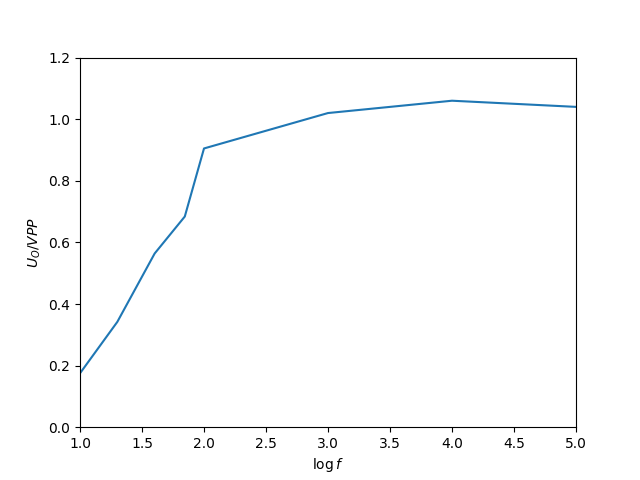
\includegraphics[width=0.60\textwidth]{幅频特性.png}
\end{figure}

由幅频特性曲线可以看出大概100-1000Hz过程输出电压的幅值达到饱和。

\subsection*{2.自举电路}
\begin{figure}[htbp]
    \centering
    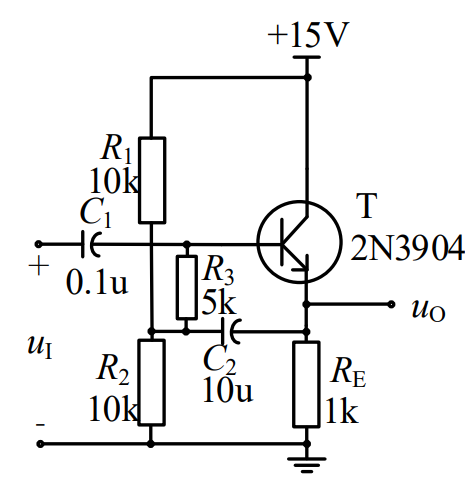
\includegraphics[width=0.35\textwidth]{电路图2.png}
    \caption{电路图2}
\end{figure}

\subsection*{(1)在 C2 加在电路中和去掉两种情况下,分别测量电路的输入电阻(加
10kHz~100kHz 之间的正弦信号,选 3 个频率点),并与仿真结果进行对比}

测量输入电阻采用实验二的方法,选用10kHz, 50kHz, 100kHz三个点,输入电压为$5mVrms$,测量外接电阻$R_1$的电压,
使用公式$R_i = \frac{U_O}{U_O' - U_O}R_1$计算输出结果。

仿真结果如下:
\begin{figure}[htbp]
    \centering
    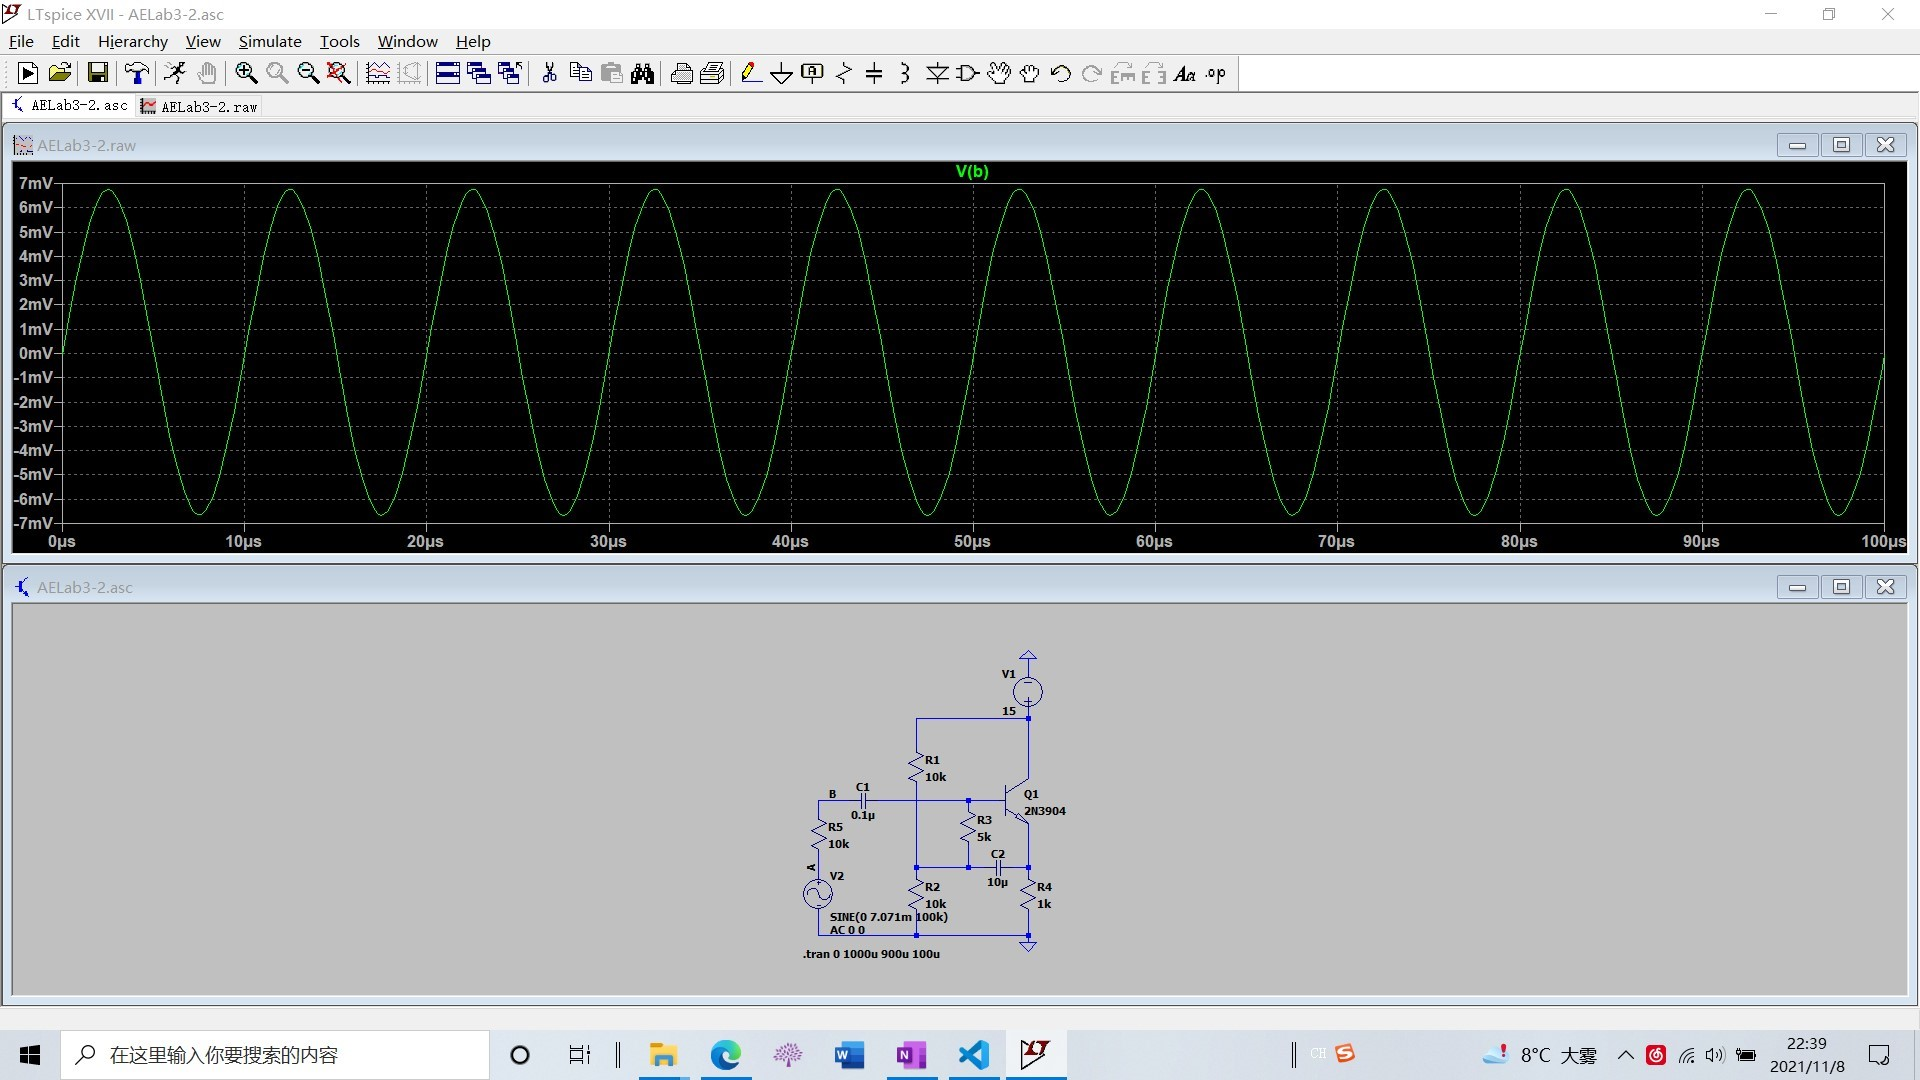
\includegraphics[width=0.60\textwidth]{2-1-10kHz.jpg}
\end{figure}
\begin{figure}[htbp]
    \centering
    \includegraphics[width=0.60\textwidth]{2-1-100kHz-无C2.jpg}
\end{figure}

仿真算出输入电阻在有$C2$时大小约为$187k \Omega$,无$C2$时为$9.5k Omega$。

实验中按照仿真所示电路连接电路。

测量结果如下:
\begin{table}[H]
    \centering
    \caption{\label{表4}\textbf{自举电路}}
    \begin{tabular}{ccccc}
    \toprule
       & $f/kHz$ & 10 & 50 & 100\\
    \midrule
        有C2 & $U_{o}/mVPP$ & 13.5 & 13.6 & 13.3\\
        & $R_i / k Omega $ & 210.9 & 251.85 & 158.33 \\
        无C2 & $U_{o}/mVPP$ & 6.9 & 6.9 & 6.8 \\
        & $R_i / k Omega $ & 9.5 & 9.5 & 9.3 \\
    \bottomrule
    \end{tabular}
\end{table}

\subsection*{(2)根据结果分析 C2 的作用}

$C_2$的作用是自举电容,它增加了输入电阻,增大了输入电压。

\end{document}